\documentclass{article}
\usepackage{graphicx}
\usepackage{url}
\usepackage{verbatim}
\usepackage{times}
\usepackage{url}
\usepackage{epsfig}
\usepackage{amsmath}

\begin{document}

\title{Technical Challenges for the RoboCup 2013 Standard Platform League Competition}

\author{RoboCup SPL Technical Committee}

\maketitle

\section{Introduction}
\label{sec:introduction}

There are three technical challenges that will be held at the RoboCup 
2013 Standard Platform League Competition. These are:

\begin{itemize}
\item The Open Challenge (Section~\ref{sec:open})
\item The Passing Challenge (Section~\ref{sec:passing})
\item The Drop-In Player Challenge (Section~\ref{sec:dropIn})
\end{itemize}

The team with the top score in a challenge will receive 25 points, each 
position thereafter will receive 1 less point; i.e. 1st = 25pts, 2nd = 24pts, 
3rd = 23pts ... 25th = 1pts. In the case of a draw, each team will receive 
the average of the points allocated to these positions; e.g. if three teams 
tie for 2nd, they will receive $(24+23+22)/3 = 23$ points. Teams not competing 
in a challenge will receive 0 points.  If a team competes in a challenge, but fails to 
score a point (or receive a vote), they will also receive 0 points. The team 
with the highest total score after all challenges is deemed the overall 
challenge winner.

All challenges will use the 2013 field and the 2013 rules will apply.  Each 
challenge will be performed in a two hour time slot, where the time slots of 
each challenge will not overlap.

\section{The Open Challenge}
\label{sec:open}
\newcommand{\openMinNum}{three}

This challenge is designed to encourage creativity within the Standard 
Platform League, allowing teams to demonstrate interesting research in 
the field of autonomous systems. Each team will be given \openMinNum{} 
minutes of time on the RoboCup field to demonstrate their research.

Each team that wishes to compete in this challenge \emph{must} send a 
short, one page document describing their demonstration to the technical 
committee by \textbf{May 27, 2013}.  Teams who do not submit this description by 
the deadline will not be allowed to compete in this challenge. These 
descriptions will be posted on the website before the competition.

The winner will be decided by a vote among all the SPL teams. In particular:

\begin{itemize}
\item 
The demonstration should be strongly related to the scope of the league. 
Irrelevant demonstrations, such as dancing and debugging tool presentations, 
are discouraged.
\item 
Each team may use any number of Aldebaran NAO robots. Teams must arrange
for their own robots.
\item 
Teams have \openMinNum{} minutes to demonstrate their research. At most one 
additional minute may be used for initial setup. Any demonstration deemed
likely to require excessive time may be disallowed by the technical
committee.
\item 
Teams may use extra objects on the field as part of their
demonstration. \emph{Robots other than the NAOs may not be used}.
\item 
The demonstration must \emph{not} mark or damage the field. Any
demonstration deemed likely to mark or damage the field may be
disallowed by the technical committee.
\item
The demonstration may \emph{not} modify the NAO robots.
\item 
The demonstration may use off-board sensors or actuators, as long 
as the NAO is still the focus of the challenge.  This is the only 
challenge in which off-board sensors or actuators are allowed.
\item 
The demonstration may use off-board computing power connected over the
wireless LAN. This is the only challenge in which off-board
computation is allowed.
\item 
The demonstration may use off-board human-computer interfaces. This
is the only challenge in which off-board interfaces, apart from the
Game Controller, are allowed.
\end{itemize}

The winner will be decided by a vote among the SPL teams using a Borda
count (\url{http://en.wikipedia.org/wiki/Borda_count}). Each SPL 
team will vote for their top 10 teams in order (excluding themselves).
Teams are encouraged to evaluate the performance based on the
following criteria: technical strength, novelty, expected impact and
relevance to RoboCup. At a time decided by the designated referee,
within one hour of the last demonstration if not otherwise
specified, the captain of each team will submit his or her team's rankings 
by filling out an online form at \url{http://goo.gl/vIVTr}.  Any points 
awarded by a team to itself will be disregarded. The points awarded by the 
teams will be summed, and the team with the highest total score shall be the winner.


\section{The Passing Challenge}
\label{sec:passing}
This challenge is intended to encourage teams to develop passing skills. In this challenge,
each team will be required to provide three robots, all robots must be in the same
colored uniform (the decision on the color of the uniforms can be made by each team).
Each robot will placed on the field inside a circle of radius 35cm (Figure \ref{fig:passing}). The center 
of the circles will be no closer then 80cm and no further then 250cm apart. The triangle formed 
by the circles will not be equilateral, i.e. the distances between robots will be different.  
The circles may be marked with a felt-tip marker (such that they are invisible to the robots) or 
with white tape (such that they may be visible to the robots).

\begin{figure}[htb]
\centering
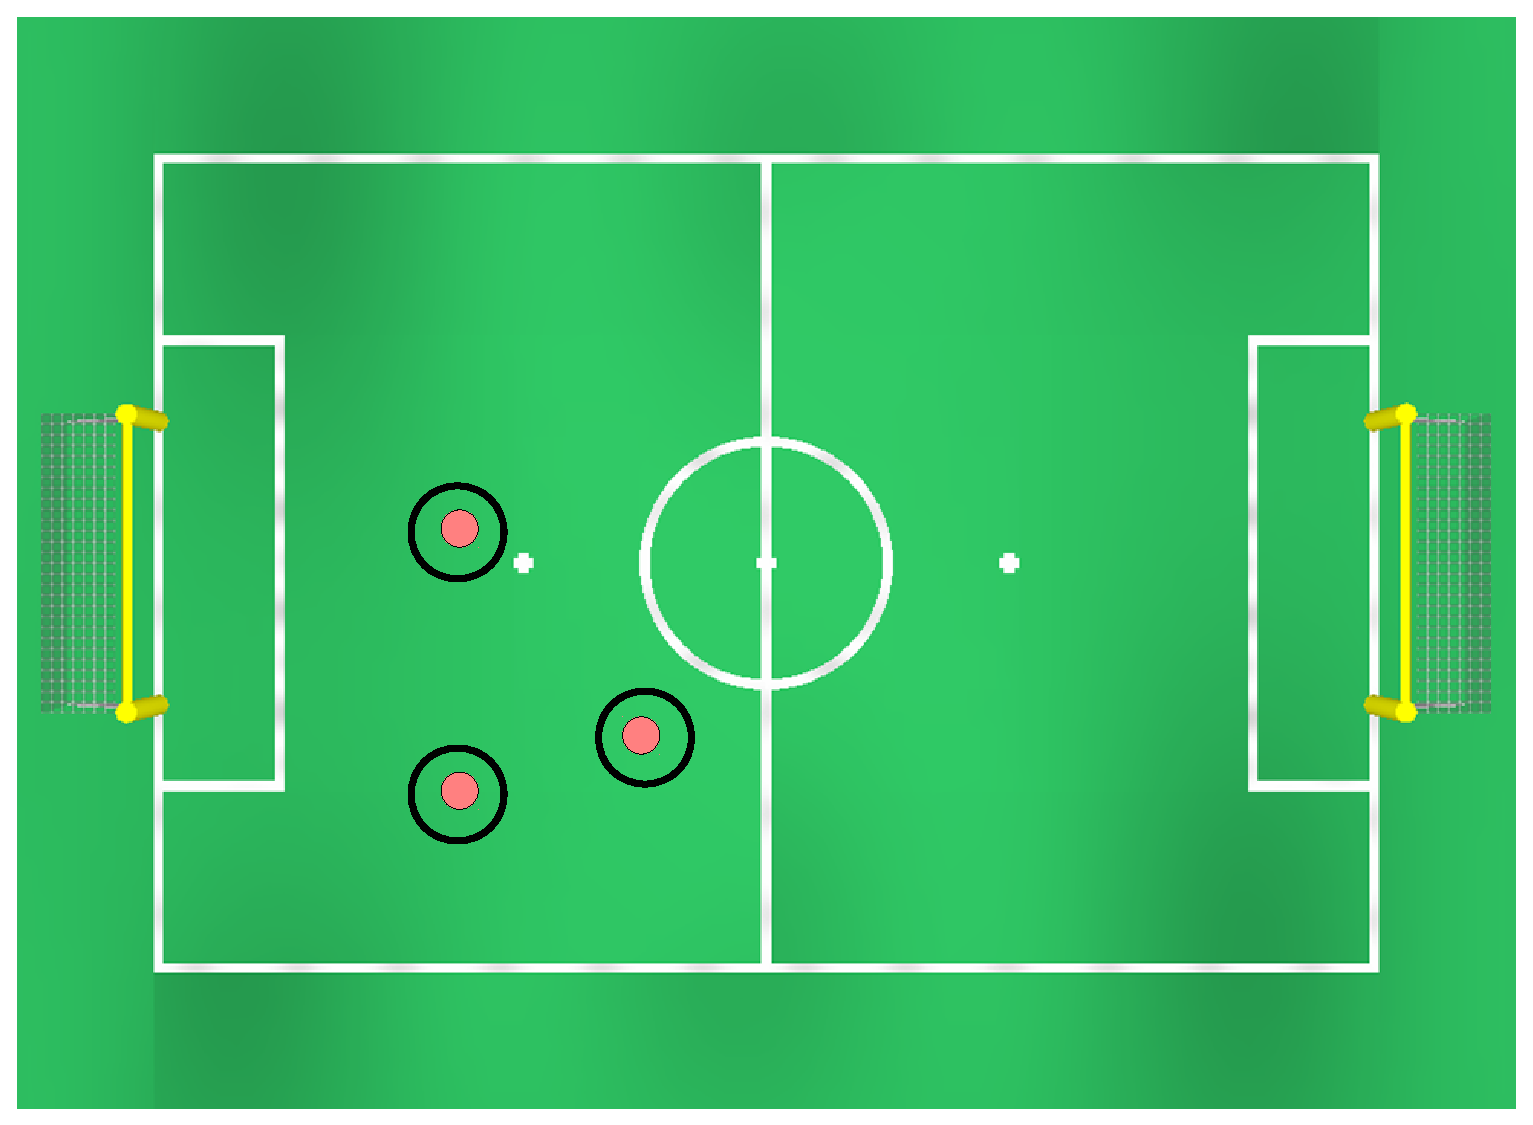
\includegraphics[width=0.6\linewidth]{figures/passing.eps}
\caption{An example placement of the robots for the passing challenge.}
\label{fig:passing}
\end{figure}

The location of the circles will be made available on the morning of the challenge.
It will be the responsibility of each team to make sure they have set the correct points.

Ten minutes before the challenge is scheduled to start, participating teams must
provide the three robots participating in the challenge to the Technical Committee 
(switched off).

Before the challenge, each robot will be booted and put into the \emph{penalized} 
state. The GameController will configure the robots to team color \emph{blue}.  Once each 
robot has been placed inside a circle, they will be placed into the `set' state for 
15 seconds. The robots will then be placed into `playing' and given three minutes to 
pass the ball around.

A pass will be regarded as successful when:
\begin{itemize}
\item The passing robot kicks the ball from inside its circle \emph{and}
\item the catching robot stops/controls the ball inside its circle. Stops/control will be
left to the referee's discretion. Examples are:
\begin{itemize}
\item The ball comes to a complete stop.
\item The robot is capable of kicking the ball from one circle to another without the need for stopping the ball.
\end{itemize}
\end{itemize}

A pass will be deemed \emph{partially} successful if:
\begin{itemize}
\item The passing robot kicks the ball from inside its circle \emph{and}
\item the catching robot touches the ball inside the circle but the ball then travels outside the circle.
\end{itemize}

A pass is deemed unsuccessful if:
\begin{itemize}
\item Either robot makes contact with the ball when the ball is outside a circle \emph{or}
\item the ball exits the field.
\end{itemize}

A robot is deemed to be inside a circle if part of one foot is inside the circle. The ball is
inside the circle if some part of the ball is inside the circle. The line is regarded as inside the circle.

Robots may pass the ball between each other in any order, but will be rewarded for passing
to a different robot then that which passed to it. Scoring of the challenge will be as
follows:
\begin{itemize}
\item \textbf{3 pts} For a successful non `return' pass that directly follows a successful pass reception.
\item \textbf{1 pt} For a successful pass.
\item \textbf{0.5 pt} For a partially successful pass.
\end{itemize}

For example, if robot 2 starts with the ball and successfully passes to robot 3, one point will be awarded.  Then if robot 3 successfully passes to robot 1, three points will be awarded.  If robot 1 then successfully passes back to robot 3, one point will be awarded.  If robot 3 then successfully passes to robot 2, three points will be awarded.  If robot 2 then has a partially successful pass to robot 1, 0.5 points will be awarded.  Then if robot 1 brings the ball back to its circle and then successfully passes to robot 3, one point will be awarded (if robot 1 had passed the ball before taking it back to its circle, no points would be awarded).

All normal game rules apply in the challenge, except:
\begin{itemize}
\item if the ball leaves the field, it will be replaced back in the closest circle
\item game stuck will not be called
\end{itemize}

If a rule is violated then any pass resulting from this violation will receive no points, and the pass itself will be considered unsuccessful.


\section{The Drop-In Player Challenge}
\label{sec:dropIn}
The main point of this challenge is for teams to develop `drop-in' players that can be good teammates and play well with a team composed of drop-in players from a variety of teams.

Each participating team will contribute one drop-in player.  Each drop-in player will compete in 5 minute games with at least three different teams composed of randomly chosen drop-in players.  In each game, the opponent will also be a team composed of randomly selected drop-in players.  The exact number of games played by each drop-in player will depend on the number of teams that participate in the challenge.

So that we can randomly draw teams and organize this challenge, each team that wishes to compete in this challenge must send a statement regarding their intent to participate in this challenge to the technical committee by \textbf{May 27, 2013}.  Teams who do not submit an intent to participate by this deadline will not be allowed to compete in this challenge.

All normal game rules apply in this challenge.  The only exception will be:
\begin{itemize}
\item Any player may be goalie (ie, enter the goal box and behave as goalie).  However, once one player has become goalie for a team, this player will be the goalie for the remainder of the game.  Any subsequent defensive players to enter the goal box will be removed as illegal defenders.
\end{itemize}

Each drop-in player may communicate with its teammates using a simple protocol.  However, drop-in players are not required to utilize this protocol.  The protocol for the communication packet is presented in pickup.h, available at \url{https://www.tzi.de/spl/pub/Website/Downloads/pickup.h}.

The challenge will be scored using two metrics: 
\begin{itemize}
\item average goal difference
\item average human judged score
\end{itemize}

The judges will likely be from other leagues, but teams are still asked to remove or cover any distinguishing markers on their robots for this challenge.  For each game, each judge will award each drop-in player a teamwork score ranging from 0 to 10, where 10 means the drop-in player was an excellent teammate and 0 means that the drop-in player ignored its teammates.  The judges will be instructed to focus on teamwork capabilities, rather than individual skills, so that a less-skilled robot could still be given top marks for good teamwork.  The human judges will help to identify good teamwork abilities in agents to ameliorate the problems of random variance in the games and the quality of teammates affecting the goal differences.

The two metrics will be normalized when determining the overall winner of this challenge.  The normalization factor will be computed to be \[\frac{10}{\text{best average goal difference of a drop-in player}}\]
Each drop-in player's average goal difference will then be multiplied by this normalization factor, to get each drop-in player's normalized average goal difference.  The normalized average goal difference will be added to the average human judged score for each drop-in player to obtain its overall score.

Each participating team should plan for at least one team member to attend the challenge.  This team member will need to update the team color and player number of their team's drop-in player between games, and potentially help referee some of the games.

\end{document}


